\section{Methodology}
\label{sec:methods}



% % \begin{figure}[t]
    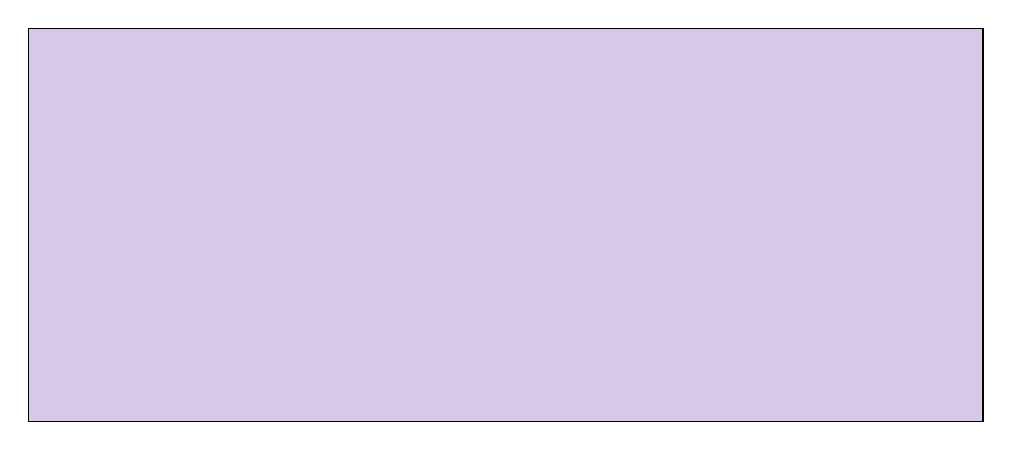
\begin{tikzpicture}
      \node[draw, fill=RoyalPurple!20, minimum width=\columnwidth, minimum height=5cm] {};
    \end{tikzpicture}
    \caption{Crawling infrastructure}
    \label{fig:infra}
    \Description["TODO: "]{"TODO"}
  \end{figure}
% \subsection{Phishing Feeds and crawling}

% We monitor Phishtank\todocite{PhishTank}, OpenPhish\todocite{OpenPhish}, PhishingDB\todocite{PhishingDB}, APWG\todocite{APWG}, and list of phishing urls from sms gateways\todocite{us or just drop this?}. 

% We crawled the pages ever 2 hours, using a automated crawler powered by the VisibleV8\todocite{VV8} patches.

% The crawler gives us insight into all javascript method calls, and property accesses, that we filter down to browser API call using the chrome idl data. 

% Our data collecting has a diverse set of techniques just at the deployment stage! docs has power-points that you have to click through to get to the page, we see a lot of blogspot, and scripts are hosted all over the place, including other phishing pages.

% \todowrite{Table of top hostnames for scripts...}
% \subsection{Data post processing}

% VisibleV8 comes with built-in post-processors that can isolate browser API calls per origin that they are called in and the URL of the script executing (in the case of a script embedded in the HTML, the origin of is the script URL).

% \subsection{Analysis}

% The provided log processors can handle isolating the browser APIs calls per origin, however, in this subsection, we describe everything else we did to isolate trends within our dataset.

% \subsubsection{MDN APIs}

% Mozilla Developer Center's Web Docs \todocite{MDN}, is documentation on different browser APIs that can be used in the modern web. The documentation breaks down the APIs into \mdncategorytotal{} categories. They also label if an API category is classified as experimental, for example, the Barcode Detection API. 

% \subsubsection{Classifying Temporal behavior}

% We describe API behavior as an increase, decrease, dip (a decrease followed by an increase), or a spike (an increase followed by a decrease).

% We first isolate out 3,978 browser APIs that show up at least in 100 web pages, we use change point detection to identify the different sections within a time series of each API. For change point detection use use ruptures\todocite{ruptures}. We use an L1 cost function along with a Linearly penalized segmentation algorithm to find the median's segmentation point of a deviation.\

% To filter out noise results, we only consider APIs with at least 2 but no more than 5 segments.

% \subsubsection{Cloaking identification}

% We manually create a list of APIs that can be used to redirect the user using client-side javascript.

% \subsubsection{First Party / Third Party identification}

% A script can be third party relative to the origin it is being loaded, or the root domain (the domain submitted). Since scripts first party to the origin can still be 3rd party scripts that are loaded in an iframe, and to minimize pollution from server-side cloaking, we consider a script first party only if it is loaded from the same domain that we aquared from our feeds.

% % \subsubsection{Kit identification}
% \subsection{Phishing behavior API categories}

% \begin{table}[t]
    
    \caption{Manual criteria to identify cloaking behavior established by Zhang \etal{}}
    \resizebox{\columnwidth}{!}{%\centering
    \begin{tabular}{cl}
        \textbf{Cloaking Category} & \multicolumn{1}{c}{\textbf{Required API calls}}                                                                                  \\ \hline
        User Interaction           & \begin{tabular}[c]{@{}l@{}}Any permission requesting API call\\ FilePicker API calls \\ HTMLElement event listeners\end{tabular} \\ \hline
        Fingerprinting             & \begin{tabular}[c]{@{}l@{}}HTMLDocument.cookie \\ HTMLDocument.referrer\\ Navigator.userAgent\end{tabular}                               \\ \hline
        Bot Behavior               & \begin{tabular}[c]{@{}l@{}}Crypto.getRandomBytes\footnote{Since Math.random is a javascript builtin function, VisibleV8 does not have visibility into it's execution}\\ Window.setTimeout + Performance.now\end{tabular}                          
        \end{tabular}
    }
\label{tab:behaviorcategories}
\end{table}

% We hand created a criteria for API to match the categories of cloaking behavior classified in Crawlphish by Zhang. \etal{}\todocite{crawlphish}. We describe the criteria for every categories for Table-\ref{tab:behaviorcategories}.

